\documentclass[%
fontsize=12pt,%
parskip=half,% 
version=last%
]{scrreprt}

% ----------------------------------------------
\usepackage[ngermanb]{babel}
\usepackage[T1]{fontenc}
\usepackage[utf8]{inputenc}

\usepackage[ngerman]{varioref} 

\usepackage{verbatim}

\usepackage{fancyvrb}

\usepackage{graphicx}

% Paket wurde wegen der Übernahme der Texte
% von pandoc geändert.
% pandoc verwedet ulem.
%\usepackage{soul}
\usepackage[normalem]{ulem}


%\usepackage{microtype}
%\usepackage{natbib}
%\usepackage{listings}
%\usepackage{fancyvrb}
%\usepackage{longtable,booktabs}
%\usepackage{graphicx}
%\usepackage{polyglossia}



\usepackage{eurosym}

\usepackage{hyperref}
\hypersetup{
  colorlinks  = true,
  pdftitle    = {Rumex Beschreibung},
  pdfsubject  = {Rumex Beschreibung},
  pdfauthor   = {Stefan Blechschmidt},
  pdfkeywords = {rumex},
  pdfcreator  = {pdflatex},
  pdfproducer = {LaTeX mit hyperref}
}


% Einbindung der htlatex Anpassung
\usepackage{rumex}


% ------------------------------------------------------
\title{Rumex Beschreibung}
\author{Stefan Blechschmidt}
\date{Juni 2014}




% ----------------------------------------------
\begin{document}

\VerbatimFootnotes

% html Konfiguration

% -------------------------------------------------
% Schalter für die Einstellungen htlatex / pdflatex
% -------------------------------------------------
\if\htorlx
%---------------------------------------------
% HTML / htlatex Lauf
%---------------------------------------------


\Css {body {width: 880px; margin:auto;}}

% Diese Anpassung wird nicht mehr gebraucht
% da die HTML Version nur mehr aus einer Seite besteht.

%% Seiten Navigation auf Deutsch umbauen 
%\Configure{crosslinks}{[}{]}{Nächste Seite}{Letzte Seite}{Letztes Seitenende}{Seitenanfang}{Seitenende} {Startseite} 
%
%% CSS Anpassung
%\Css {.crosslinks { font-size: 0.9em; padding-left:1em; background-color: \#eee; border: 1px solid gray;}}
%\Css {p {font-size: 1.2em;}}
%\Css {.sectionTOCS:before { display: block; content: 'Unterabschnitte:'; color: gray; padding-bottom: 8px; }}
%\Css {.sectionTOCS {font-size: 1.1em; border-top: 1px solid silver; border-bottom: 1px solid silver; padding: 1em 0;}}
%\Css {.sectionHead {padding-top:2em;}}
%\Css {.tableofcontents:before { display: block; content:
%'Inhaltsverzeichnis:'; color: gray; padding-bottom: 8px; }}
%\Css {.tableofcontents {border-top: 1px solid silver; border-bottom: 1px
%solid silver; padding: 1em 0 1em 1em;}}
%\else
%---------------------------------------------
% LaTeX Lauf
%---------------------------------------------

\fi

% ENDE Schalter für htlatex / pdflatex Einstellungen

\maketitle

\begin{abstract}
An diesem Dokument wird zur Zeit gearbeitet.
\end{abstract}


\section{Vorwort}\label{vorwort}

Die Beweggründe mit einem eigenen System eine Internet Seite zu
Verwalten sind mit der Zeit in mir gewachsen.

Es gibt immer mehr Systeme die zum Erstellen und Verwalten von
Internetseiten eingesetzt werden. Probiert habe ich schon viele und mit
den meisten war ich auch sehr zufrieden, wenn da nicht immer der Hacken
mit dem Updates wäre. Irgendwie, zumindest kommt es mir so vor, ist der
Aufwand das System der Seite auf dem aktuellen Stand zu halten größer
geworden als den Inhalt der eigentlichen Seite zu pflegen.

Ich wünschte mir wieder eine Internetseite wie in früheren Zeiten. Eine
Seite die aus einfachen HTML Seiten besteht.

Irgendwann bin ich dann auf \texttt{markdown} und \texttt{pandoc}
gestoßen und die Idee dieses Home Page Baukastens ist entstanden.

\subsection{Rumex?}\label{rumex}

Rumex ist die lateinische Bezeichnung für den
\href{http://de.wikipedia.org/wiki/Ampfer}{Ampfer} und dieser taucht in
der Natur dann auf, wenn der Boden Überdüngt, Verdichtung und Beschädigt
ist. Rumex gehört zu den sogenannten Pionier Pflanzen. Er ist ein
Lückenfüller.

Genau das soll Rumex auch sein ``ein Lückenfüller'' für alle die
\ldots{} Systeme satt haben.

\begin{figure}[htbp]
\centering
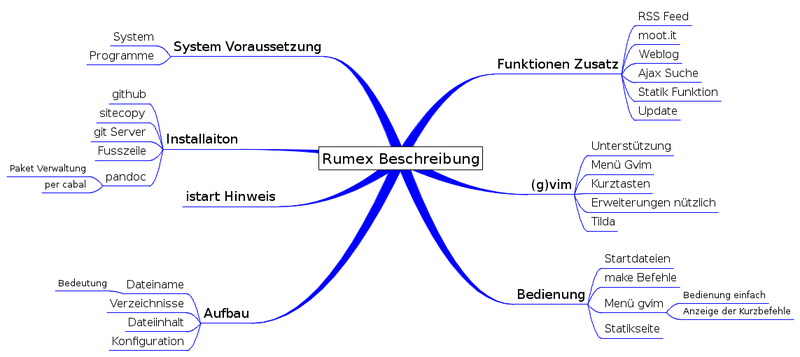
\includegraphics{../bilder/beschreibung-vym_800_.png}
\caption{Kleine Gedankenkarte der Rumex Beschreibung. Zur Zeit in
Arbeit.}
\end{figure}

\section{Installation und Einrichten des Rumex
Baukastens}\label{installation-und-einrichten-des-rumex-baukastens}

\subsection{Vorbereitung des Rechners}\label{vorbereitung-des-rechners}

Rumex ist auf ein *nix System ausgerichtet. Auf diesem sollten folgende
Programme installiert sein:

\begin{itemize}
\item
  bash
\item
  make
\item
  perl
\item
  git
\item
  pandoc
\item
  imagemagick
\item
  wget
\item
  \sout{wput}
\item
  sitecopy
\item
  vim (g)vim
\item
  texlive
\end{itemize}

Wobei \texttt{bash}, \texttt{make} und \texttt{perl} eigentlich bei
jeder \texttt{*nix} Installation bereits vorhanden sein dürft. Die
restlichen Programme müssen nach installiert werden.

Wer mit dem Editor \texttt{vim} zurecht kommt sollte sich auch
\texttt{(g)vim} installieren. Rumex besitzt eine \texttt{gvim}
Erweiterung die, die Arbeit bzw. die Suche nach dem richtigen Befehl am
Anfang um einiges erleichtert.

\texttt{texlive}\footnote{Die Funktion der PDF Erstellung ist zur Zeit
  noch nicht enthalten.} wird nur gebraucht wenn man auch PDF Dateien
erstellen möchte.

\sout{\texttt{wput}} \texttt{sitecopy} wird nur gebraucht wenn man die
Daten per FTP hoch laden möchte.

\begin{verbatim}
sudo apt-get install make perl

sudo apt-get install git-core wget sitecopy pandoc imagemagick

sudo apt-get install gvim

sudo apt-get install texlive
\end{verbatim}

\subsection{Installation von Rumex auf dem lokalen
Arbeitsplatz}\label{installation-von-rumex-auf-dem-lokalen-arbeitsplatz}

Für die Installation auf deinem Rechner musst du dir zu erst das ZIP
bzw. das tar.gz Archiv vom github Server holen und entpacken

\begin{verbatim}
wget https://github.com/itbayer/rumex/archive/gh-pages.zip
unzip gh-pages.zip
\end{verbatim}

oder

\begin{verbatim}
wget https://github.com/itbayer/rumex/archive/gh-pages.tar.gz
tar -xzvf gh-pages.tar.gz
\end{verbatim}

Jetzt wechsle in das Verzeichnis \texttt{rumex-gh-pages/.rx} und starte
die Befehle \texttt{make install} und \texttt{make show}.

\begin{verbatim}
cd rumex-gh-pages/.rx/
make install
make show
\end{verbatim}

Fertig :-)

\subsection{Rumex auf dich einstellen}\label{rumex-auf-dich-einstellen}

Nach der Installation muss Rumex noch auf dich eingestellt werden.
Genauer gesagt sollten folgende Angabe für deine neuen Seite angepasst
werden.

\begin{itemize}
\itemsep1pt\parskip0pt\parsep0pt
\item
  URL deiner Seite
\item
  Impressum
\item
  Kopf / Fusszeile
\item
  Logo
\end{itemize}

Eine Kurzbeschreibung findest du, nach der Installation, auf der
Startseite von Rumex oder \href{../istart.html}{hier}.

\subsection{moot.it}\label{moot.it}

@todo: Hier fehlt noch die Beschreibung

\begin{itemize}
\itemsep1pt\parskip0pt\parsep0pt
\item
  ein/auschalten
\item
  Kontoname einstellen
\end{itemize}

\subsection{gvim Unterstützung
einrichten}\label{gvim-unterstuxfctzung-einrichten}

@todo: Hier fehlt noch die Beschreibung@

\begin{itemize}
\itemsep1pt\parskip0pt\parsep0pt
\item
  Erstellen der Startdatei
\item
  Einrichten
\end{itemize}


% Dieser Teil wurde ausgeblendet da bei der Übernahme
% von Pandoc noch Fehler auftreten

%\subsubsection{AutoSave Funktion}\label{autosave-funktion}
%
%Mit dem Plugin AutoSave kann man Rumex auch dazu bringen Dateien nicht
%nur automatisch zu speichern sondern auch gleich die HTML Datei zu
%erstellen.
%
%Jedoch ist eine kleine Änderung am Plugin notwendig.
%
%\begin{Shaded}
%\begin{Highlighting}[]
%\KeywordTok{diff --git a/plugin/AutoSave.vim b/plugin/AutoSave.vim}
%\NormalTok{index f09a904..ec2f463 100644}
%\DataTypeTok{--- a/plugin/AutoSave.vim}
%\DataTypeTok{+++ b/plugin/AutoSave.vim}
%\DataTypeTok{@@ -11,6 +11,12 @@ else}
%   \NormalTok{let g:auto_save_loaded = 1}
% \NormalTok{endif}
% 
%\OtherTok{+if exists("g:rumex")}
%\OtherTok{+  finish}
%\OtherTok{+else}
%\OtherTok{+  let g:rumex = 0}
%\OtherTok{+endif}
%\OtherTok{+}
% \NormalTok{let s:save_cpo = &cpo}
% \NormalTok{set cpo&vim}
% 
%\DataTypeTok{@@ -33,10 +39,14 @@ function! AutoSave()}
%   \NormalTok{if g:auto_save >= 1}
%     \NormalTok{let was_modified = &modified}
%     \NormalTok{silent! wa}
%\StringTok{-    if was_modified && !&modified}
%\StringTok{-      echo "(AutoSaved at " . strftime("%T") . ")"}
%\StringTok{-    endif}
%\StringTok{-  endif}
%\OtherTok{+   if was_modified && !&modified}
%\OtherTok{+       if g:rumex == 1}
%\OtherTok{+           silent! make html}
%\OtherTok{+           echo "html datei wurde erstellt"}
%\OtherTok{+       endif}
%\OtherTok{+       echo "(AutoSaved at " . strftime("%T") . ")"}
%\OtherTok{+   endif}
%\OtherTok{+endif}
% \NormalTok{endfunction}
% 
% \NormalTok{function! AutoSaveToggle()}
%\end{Highlighting}
%\end{Shaded}
%
%Mit dem Befehl \texttt{:let rumex=1} bzw. \texttt{let rumex=0} kann das
%Erstellen der HTML Datei ein bzw. ausgeschaltet werden.
%
%Installiert man sich dann noch im FireFox dann noch die Erweiterung.
%``Tab Auto Reload'' werden die Änderungen im Browser immer gleich
%angezeigt.
%
%Über die Nutzbarkeit kann man sich streiten da nach einem HTML Lauf der
%Cursor immer an den Anfang der Zeile, in der man sich gerade befindet,
%springt. Mir ist die Variante mit \texttt{\textless{}F5\textgreater{}}
%lieber. Die ``Tab Auto Reload'' Funktion im Firefox verwende ich aber
%schon sehr gerne.

\subsubsection{Tipps zur Benutzung gvim}\label{tipps-zur-benutzung-gvim}

\subsubsection{vim Kurztasten}\label{vim-kurztasten}

Eine Übersicht der Rumex Kurztasten für den Editor vim findest du auf
der Seite \href{vim-kurztasten.htm}{VIM-Kurztasten}.

\subsubsection{gvim Menü}\label{gvim-menuxfc}

Eine Übersicht des Rumex Menüs für den Editor gvim findest du auf der
Seite \href{gvim-menue.htm}{GVIM-Menü}.

\paragraph{Dateiname ergänzen}\label{dateiname-erguxe4nzen}

Will man in die Datei einen Dateinamen einbauen, weiß aber nicht mehr
genau wie er heißt, kann man folgenden Trick verwenden. In diesem
Beispiel wird ein Bildname gesucht. Im Text schreibe man
\texttt{../bilder/tw} und drückt dann die Tastenkombination
\texttt{C-X + C-F}, gvim öffnet ein Dialogfeld in dem alle Dateien die
auf dieses Muster übereinstimmen geöffnet. Gibt es nur einen Treffer
wird dieser gleich eingefügt.

\paragraph{Wort innerhalb des Dokumentes
suchen}\label{wort-innerhalb-des-dokumentes-suchen}

Sucht man ein Wort das man im Dokument schon einmal verwendet hat, um
zum Beispiel darauf zu verweisen. Schreibt man den Wortanfang und drückt
dann \texttt{C-P}. Es öffnet sich ein Dialogfeld in dem alle Wörter die
auf dieses Muster passen angezeigt werden. Gibt es nur einen Treffer
wird dieser gleich eingefügt.

\paragraph{Nützliche Erweiterungen}\label{nuxfctzliche-erweiterungen}

Vim bietet ein paar nützliche Erweiterungen in Form von plugins an. Hier
eine Liste, der plugins, die ich gerne verwende.

\begin{description}
\item[pathogen.vim]
Diese Erweiterung macht das Installieren weitere Erweiterungen einfach.
Dabei ist die Installation von \texttt{pathogen} schnell erledigt.

%\begin{Shaded}
%\begin{Highlighting}[]
%\KeywordTok{mkdir} \NormalTok{-p ~/.vim/autoload ~/.vim/bundle }
%\KeywordTok{wget} \NormalTok{-O ~/.vim/autoload/pathogen.vim //}
%\KeywordTok{http}\NormalTok{://www.vim.org/scripts/download_script.php?src_id=16224}
%\end{Highlighting}
%\end{Shaded}

In die \texttt{.vimrc} muss dann noch nachfolgende Zeile eingebaut
werden.

\begin{verbatim}
call pathogen#infect()
\end{verbatim}

eingebaut werden.

Jetzt braucht man die Erweiterungen nur mehr in das Verzeichnis
\texttt{.vim/bundle} zu kopieren und vim neu starten. In Verbindung mit
\texttt{git} wieder eine einfache Sache.

%\begin{Shaded}
%\begin{Highlighting}[]
%\KeywordTok{cd} \NormalTok{~/.vim/bundle}
%\KeywordTok{git} \NormalTok{clone https://github.com/vim-pandoc/vim-pandoc.git}
%\end{Highlighting}
%\end{Shaded}

\item[vim-pandoc]
Erweiterung rund um pandoc.
\item[FuzzyFinder]
Dateien schnell zum editieren öffnen. Installiert ist diese Erweiterung,
vorausgesetzt man verwendet pathogen, mit dem Befehl:

\begin{verbatim}
wget -O /tmp/vim-fuzzyfinder.zip http://www.vim.org/scripts/download_script.php?src_id=10588
mkdir ~/.vim/bundle/vim-fuzzyfinder
unzip /tmp/vim-fuzzyfinder.zip -d ~/.vim/bundle/vim-fuzzyfinder/
\end{verbatim}

Für das öffnen dies Datei Dialogs sollte man sich dann noch eine
Kurztaste konfigurieren.

\begin{verbatim}
" -------------------------------------------------------------
" FuzzyFinder File Suche auf <F12> binden
map <F12> :FuzzyFinderFile <CR>
\end{verbatim}
\end{description}

\subsection{Seite auf einem github.com Server
einrichten}\label{seite-auf-einem-github.com-server-einrichten}

@todo

\begin{itemize}
\itemsep1pt\parskip0pt\parsep0pt
\item
  Einrichten eines github.com Zugangs
\item
  Arbeits- Repository auf den AP\footnote{Mit AP ist der
    \textbf{A}rbeits\textbf{P}latz Rechner gemeint.} holen
\item
  Die Rumex ZIP Datei
\item
  Die Dateien des ZIP Archives in das Arbeits- Repository kopieren
\item
  Grund Dateien anpassen

  \begin{itemize}
  \itemsep1pt\parskip0pt\parsep0pt
  \item
    @fixme: Angabe welche Dateien fehlt noch@
  \end{itemize}
\item
  Erste Änderungen vornehme
\item
  \texttt{make online} - Fertig.
\end{itemize}

\subsection{Seite auf einem nicht github.com Server
einrichten}\label{seite-auf-einem-nicht-github.com-server-einrichten}

\subsubsection{Datei upload per git}\label{datei-upload-per-git}

@todo

Auf der Seite \href{http://rumex.it-bayer.de}{rumex.it-bayer.de} findet
man eine Beschreibung wie man den rumex Baukasten auf einen
\textbf{nicht} \texttt{github.com} Server installiert.

\subsubsection{Datei upload per ftp}\label{datei-upload-per-ftp}

@todo

\section{Aufbau des rumex Baukastens}\label{aufbau-des-rumex-baukastens}

@todo

\subsection{root Verzeichnis}\label{root-verzeichnis}

Im \texttt{root} Verzeichnis findet man alle \texttt{HTML} Dateien der
Seite. Diese werde vom Baukasten erstellt und müssen nicht von Hand
verändert werden. Zusätzlich findet man noch ein folgende Systemdateien:

\begin{description}
\item[rss.xml]
News Feed Datei, wird vom System erstelle
\item[readme.md]
Beschreibungsdatei die von github.com gebraucht wird
\item[robots.txt]
Datei für die Suchmaschinen
\item[favicon.ico]
Icon für den Browser
\item[.htaccess]
Konfiguration für den Apache Server
\item[CNAME]
@fixme: Beschreibung@
\end{description}

\subsection{Unterverzeichnisse}\label{unterverzeichnisse}

\begin{description}
\item[.rumex/]
@fixme: Beschreibung@
\item[.rx/]
@fixme: Beschreibung@
\item[rxtpl/]
Standard Template Verzeichnis. In diesem Verzeichnis befinden sich die
Dateien die für das Aussehen der Seite verantwortlich sind.

Folgende Dateinen und Verzeichnisse sind hier zu finden

\begin{itemize}
\itemsep1pt\parskip0pt\parsep0pt
\item
  index.html (Weiterleitung zum root Verzeichnis)
\item
  css/\\
\item
  js/
\item
  img/
\end{itemize}
\item[bilder/]
In diesem Verzeichnis werden alle Bilder der Seite abgelegt.
\end{description}

\subsection{Steuerung durch
Dateiendung}\label{steuerung-durch-dateiendung}

Das Aussehen der Dateien bezüglich des Inhaltsverzeichnisses könnte auch
durch die Dateiendung gesteuert werden.

\subsubsection{Beispiel}\label{beispiel}

\begin{description}
\item[datei.rx0s]
Würde eine HTML Datei ohne Inhaltsverzeichnis erstellen.
\item[datei.rx1s]
Erstellt die HTML Datei mit dem Inhaltsverzeichnis aus den Einträgen der
H1 Überschriften.
\item[datei.rx2s]
Erstellt eine HTML Datei mit dem Inhaltsverzeichnis aud den Einträgen
der H1 und H2 Überschriften.
\end{description}

Zusätzlich könnte die Dateiendung auch eine unterschiedliche Verwendung
der Dateien ermöglichen.

\begin{description}
\item[datei.rx0s, datei.rx1s \ldots{}]
Standard Datei.
\item[datei.rx0x, datei.rx1x \ldots{}]
Datei die nicht in die Liste auf \texttt{index.html} eingebunden wird.
\item[datei.rx0v, datie.rx1v \ldots{}]
Versteckte Datei. Diese taucht weder in der \texttt{index.html} noch in
der \texttt{sitemap.xml} auf.
\item[datei.rx0w]
Datei mit einer Weiterleitung. Die Weiterleitung wird dabei mittels
\texttt{javascript} realisiert, da github keine \texttt{.htaccess}
Weiterleitung unterstützt.

\begin{verbatim}
% Weiterleitung nach beschreibung.html
%
%

<script language="javascript">
<!--
window.location.href="beschreibung.html";
// -->
</script> 
\end{verbatim}
\end{description}

Bei der Änderung der Dateiendung bleibt der eigentliche \texttt{html}
Name gleich. Nur die Funktion der Einbindung ändert sich.

\subsection{Sonderseiten}\label{sonderseiten}

Im Verzeichnis \texttt{pandoc} befinden sich Sonderseiten.

\begin{description}
\item[rumex/index.rx0x]
Diese Datei wird vom Programm \texttt{.bin/make\_index.pl} erstellt,
muss somit nicht vorhanden sein.
\item[rumex/start.rx0s]
Die \texttt{start.rx0s} wird als Vortext in die \texttt{index.rx0x}
eingebunden. Mit ihr kann man oberhalb der Seiten Liste einen extra Text
in die \texttt{index.html} eingebunden werden.\\\textbf{Diese Datei ist
erforderlich und muss vorhanden sein.}
\item[rumex/rss.rx0x]
Datei für die RSS Feed Funktion.
\item[rumex/impressum.rx0x]
Datei für die Impressumsangaben.\\\textbf{Ist nicht zwingend
erforderlich. Jedoch muss die \texttt{.inc/fuss.html} entsprechende
bearbeitet, der Link muss raus genommen, werden.}
\item[rumex/Makefile]
Sie \texttt{make} Steuerdatei.
\end{description}

\subsection{Aufbau der Startseite}\label{aufbau-der-startseite}

Die Startseite \texttt{markdown/start.rx0s} muss vorhanden sein. Es
reicht auch ein `touch markdown/start.rx0s.

Der normale Aufbau könnte so ausschauen. Die \texttt{pandoc} Kopfzeile
sind nicht zwingend erforderlich.

\begin{verbatim}
% start.rx0s
%
%

Hier kommt auch schon der Vortext für die index.html
\end{verbatim}

\subsection{Aufbau der Einzelseiten}\label{aufbau-der-einzelseiten}

Die Einzelseiten liegen alle im Verzeichnis \texttt{rumex} und zwar in
der Sprache \texttt{markdown} bzw. der Erweiterung von \texttt{pandoc}.

Diese Einzelseiten werden in chronologischer Reihenfolge in die
Startseite \texttt{index.html} eingebunden und bilden sozusagen das
Inhaltsverzeichnis der Seite. In jeder Einzelseite wird dazu ein
sogenannter \emph{``Vortext''} hinterlegt. Die Seite bzw. der Kopf der
Seite hat dabei folgenden Aufbau.

\begin{verbatim}
% Seiten Überschrift 1
% Seiten Überschrift 2
% Seiten Überschrift 3

<!--


# Listen-Überschrift

Überschrift und Text der in der Listenübersicht
auf index.html angezeigt wird.

Alles was innerhalb der HTML Kommentar Marken
steht wird nur auf der index.html Seite angezeigt.

-->

Alles was sich außerhalb der HTML Marken
befindet wird auch auf der eigentlichen Seite angezeigt.

Durch das Schlüsselwort "schnipp", das auch in HTML
Kommentar Marken stehen muss, wird der Vortext beendet.
Auf der index.html erscheint an dieser Stelle der Link
"... weiter lesen".

<!-- schnipp -->

Ab hier geht dann der Inhlat der eigentlichen Seite los.
\end{verbatim}

\subsection{Template}\label{template}

@todo

Änderung gegenüber des Original \texttt{pandoc} Templates.

%\begin{Shaded}
%\begin{Highlighting}[]
%\DataTypeTok{5c5,8}
%\StringTok{<   <meta name="generator" content="pandoc">}
%\KeywordTok{---}
%\OtherTok{>   <!-- rumex Version -->}
%\OtherTok{>   <meta name="generator" content="$meta_generator$">}
%\OtherTok{>   <!-- rumex Suchmaschine -->}
%\OtherTok{>   <meta name="robots" content="$meta_robots$">}
%\DataTypeTok{30a34,35}
%\OtherTok{>   <!-- rumex RSS -->}
%\OtherTok{>   <link rel="alternate" type="application/rss+xml" title="$rsstitel$" href="$rssfile$" />}
%\DataTypeTok{41c46}
%\StringTok{< <h1 class="title">$title$</h1>}
%\KeywordTok{---}
%\OtherTok{> <h1 class="title"><a title="zur Startseite" href="index.html">$title$</a></h1>}
%\DataTypeTok{43c48}
%\StringTok{< <h2 class="author">$author$</h2>}
%\KeywordTok{---}
%\OtherTok{> <h2 class="author"><a title="zur Startseite" href="index.html">$author$</a></h2>}
%\DataTypeTok{46c51}
%\StringTok{< <h3 class="date">$date$</h3>}
%\KeywordTok{---}
%\OtherTok{> <h3 class="date"><a title="zur Startseite" href="index.html">$date$</a></h3>}
%\DataTypeTok{54a60}
%\OtherTok{> <div id=seite>}
%\DataTypeTok{55a62}
%\OtherTok{> </div>}
%\end{Highlighting}
%\end{Shaded}

\section{RSS Feed Funktion}\label{rss-feed-funktion}

@todo

Wird nicht aus den einzelnen Dateien erstellt sondern muss manuell
editiert werden, Datei \texttt{.rx/rss.rx0x}.

Jede Überschrift eines Eintrags muss mit einem \texttt{\{.nn1\}} enden.

Danach kommen die Angaben zu:

\textbf{Link:} \emph{Verweis zur Seite mit weiteren
Informationen}\\\textbf{Autor:} \emph{Autor der den Eintrag geschrieben
hat}\\\textbf{Kategorie:} \emph{Kategoie des Eintrags}\\\textbf{Datum:}
\emph{Datum des Eintrags.} Das richtige Format bekommt man mit dem
Befehl \texttt{date -R}.

die in HTML Kommentar Marker eingeschlossen sind.

Anschließend folgt die Meldung. Zur Zeit werden folgende \texttt{pandoc}
Formatierungen unterstützt.

\begin{itemize}
\itemsep1pt\parskip0pt\parsep0pt
\item
  Überschriften ab der Stufe 3 \texttt{\#\#\#}
\item
  Aufzählungen \texttt{-}
\item
  Aufzählungen \texttt{*}
\item
  Zitate \texttt{\textgreater{}}
\item
  Links \texttt{{[}Link{]}(http://muster.tdl)}. Diese dürfen nicht am
  Anfang einer Zeile stehen.
\item
  Bilder \texttt{!{[}Bild{]}(../bilder/muster.png "muster.png")}, Diese
  dürfen nicht am Anfang einer Zeile stehen.
\item
  Code `Code`.
\end{itemize}

\subsection{Beispiel einer RSS Feed
Seite}\label{beispiel-einer-rss-feed-seite}

%\begin{Shaded}
%\begin{Highlighting}[numbers=left,,firstnumber=100,]
% \NormalTok{% Abo Seite - Newsletter - RSS Feed}
% \NormalTok{% }
% \NormalTok{%}
% 
% \NormalTok{<!--}
% \NormalTok{| Titel: Rumex - Ein Home Page Baukasten}
% \NormalTok{| Beschreibung: Aktuelles und Neuigkeiten vom rumex Home Page Baukasten}
% \NormalTok{| KLink: http:}\CommentTok{//www.it-bayer.de/rumex/}
% \NormalTok{| Lang: de-DE}
% \NormalTok{| BildTitel: IT-Bayer rumex Meldungen}
% \NormalTok{| BildURL: http:}\CommentTok{//www.itbayer.de/rumex/bilder/404.png}
% \NormalTok{| BildLink: http:}\CommentTok{//www.it-bayer.de/rumex/}
% \NormalTok{| BildBeschreibung: Aktuelles und Neuigkeiten von der rumex Seite.}
% \NormalTok{-->}
% 
% \ErrorTok{# rumex bekommt die RSS Feed Funktion\{.rssfeed1\}}
% 
% \NormalTok{<!-- }
% \NormalTok{| Link: http:}\CommentTok{//www.it-bayer.de/rumex/}
% \NormalTok{| Autor: IT-Bayer}
% \NormalTok{| Kategorie: Neues}
% \NormalTok{| Datum: Thu, }\DecValTok{04} \NormalTok{Jul }\DecValTok{2013} \DecValTok{10}\NormalTok{:}\DecValTok{07}\NormalTok{:}\DecValTok{06} \NormalTok{+}\DecValTok{0200}
% \NormalTok{-->}
% 
% \NormalTok{In den rumex Baukasten wurde eine RSS Feed Funktion eingebaut.}
% \NormalTok{Die Einträge werden dabei auch aus einem `pandoc` Dokument gelesen}
% \NormalTok{und nach `rss.xml` geschrieben.}
% 
% \NormalTok{Zusätzlich ist diese Datei auch als `rss.html` unter }
% \NormalTok{<http:}\CommentTok{//www.it-bayer.de/rumex/rss.html> verfügbar.}
%\end{Highlighting}
%\end{Shaded}

\subsection{RSS Dateiname}\label{rss-dateiname}

Der Dateiname ist mit \texttt{rss.xml} vorbelegt und kann über die
Variable \texttt{RSS\_FILE} in der \texttt{config.md} geändert werden.

\subsection{RSS Titel}\label{rss-titel}

Der Title des RSS Feed wird durch die Variable \texttt{RSS\_TITEL}
angepasst.

\begin{verbatim}
RSS_TITEL = "Neuigkeiten von rumex Baukasten"
\end{verbatim}

\subsection{RSS auslagern}\label{rss-auslagern}

Den RSS Link kann man auch auslagern so dass dieser auf eine andere
Seite zeigt. Dazu setzt man die Variable \texttt{RSS\_EXTERN} mit dem
entsprechenden Link. Die Variabel \texttt{RSS\_FILE} wird dadurch nicht
mehr verwendet. Auch der RSS Lauf wird dadurch ausgeschaltet und durch
eine Meldung ersetzt.

\subsection{RSS Kurztaste}\label{rss-kurztaste}

Für die einzelnen Einträge steht auch eine Kurztaste \texttt{.rnn} zur
Verfügung.\\In Gvim unter

\begin{verbatim}
Rumex -> TextBausteine -> NeuerNews Eintrag
\end{verbatim}

Eingefügt wird dann folgende Vorgabe. Der Wert hinter Datum wird von
System ausgelesen und entsprechende gesetzt.

\begin{verbatim}
 # Neue Nachricht{.nn1}

<!--
| Link: http://www.it-bayer.de/rumex/
| Autor: IT-Bayer
| Kategorie: Neues
| Datum: Mon, 28 Oct 2013 07:36:56 +0100
-->

Ab hier geht die neue Nachricht los.
\end{verbatim}

\subsection{Interna}\label{interna}

Durch die beschriebenen RSS Variablen wird die Erstellung des RSS Feed
gesteuert. Es wird in jede HTML Datei nachfolgender Header Abschnitt
eingebaut wenn die \texttt{RSS\_TITLE} Variable gesetzt wurde.
\texttt{RSS\_FILE} bzw. \texttt{RSS\_EXTERN} steuern den \texttt{href}
Eintrag.

%\begin{Shaded}
%\begin{Highlighting}[]
%\CommentTok{<!-- rumex RSS -->}
%\KeywordTok{<link}\OtherTok{ rel=}\StringTok{"alternate"}\OtherTok{ type=}\StringTok{"application/rss+xml"}\OtherTok{ title=}\StringTok{"Neuigkeiten von rumex Baukasten"}\OtherTok{ href=}\StringTok{"rss.xml"} \KeywordTok{/>}
%\end{Highlighting}
%\end{Shaded}

\section{Rumex auf einem USB Stick}\label{rumex-auf-einem-usb-stick}

Rumex kann auch auf einem USB Stich installiert werden. Der Stick muss
aber ein Dateiformat besitzt\\welches mit Dateirechten und Symbolische
Links umgehen kann.

\textbf{USB Sticks im VFAT Format funktionieren nicht.} Man kann zwar
die Daten darauf ablegen. Das Arbeiten über den Stick funktioniert nicht
wirklich. Auch wenn man die Daten, von einem VFAT Stick, auf ein *nix
System kopiert werden muss händisch nach gebessert werden.

LinkTipp:
\href{http://www.it-bayer.de/usb-stick.html?suchwort=versch\#usb-stick-unter-linux-verschl\%C3\%BCsseln}{USB
Stick unter Linux verschlüsseln}

\section{make Steuerung}\label{make-steuerung}

@todo

Gesteuert wird der Baukasten mittels \texttt{make} im Unterverzeichnis
\texttt{rumex}. Folgende \texttt{make} Befehle stehen dabei zur
Verfügung.

\begin{description}
\item[make html]
Erstellt die einzelnen html Dateien. Hier kann auch nur \texttt{make}
verwendet werden.
\item[make index]
Erstellt die \texttt{index.md} Datei aus der dann die
\texttt{index.html} Datei erstellt wird.
\item[make all]
Eine Zusammenstellung aus \texttt{make index} und \texttt{make html}.
\item[make online]
Daten auf github hoch laden.
\item[make bilder]
Erstellt Bilder in verschiedenen Auflösungen.
\end{description}

\section{Update}\label{update}

@todo

\section{Homepage Änderung, schnell und immer
aktuell}\label{homepage-uxe4nderung-schnell-und-immer-aktuell}

Wer wünscht es sich nicht einen schnellen Zugriff auf seine Homepage.
Sei es um schnell was zu ändern oder genauso schnell was neues
einzustellen. Rumex bietet in Verbindung mit \texttt{tilda} eine schöne,
einfache und auch schnelle Lösung.

\begin{figure}[htbp]
\centering
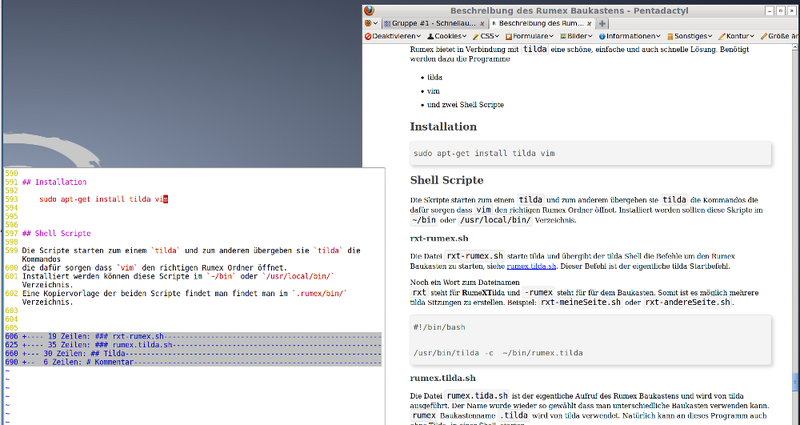
\includegraphics{../bilder/rumex-tilda_800_.png}
\caption{Rumex im tilda Fenster. Mit einem Tastendruck öffnet sch das
tilda Fenster und man kann die Texte eintippen. Ein erneuter Tastendruck
schließt das tilda Fenster wieder und der Bildschirm ist wieder frei.
Hat man seine Änderung abgeschossen kann man mit den Rumex
\href{vim-kurztasten.html}{vim Kurztasten} die Änderung schnell online
stellen.}
\end{figure}

\subsection{Installation der tilda
Unterstützung}\label{installation-der-tilda-unterstuxfctzung}

Die Installation ist nicht umfangreich. Man braucht vim und tilda und
dann noch zwei bash Script. Eine Kopiervorlage der beiden Scripte findet
man findet man im \texttt{.rumex/bin/} Verzeichnis.

\begin{verbatim}
sudo apt-get install tilda vim
cp .../rumex/.rumex/bin/rxt-rumex.sh ~/bin/.
cp .../rumex/.rumex/bin/rumex-tilda.sh ~/bin/.
\end{verbatim}

Diese beiden bash Scripte müssen anschließend noch angepasst werden.

\subsubsection{Shell Scripte}\label{shell-scripte}

Die Scripte starten zum einem \texttt{tilda} und zum anderem übergeben
sie \texttt{tilda} die Kommandos die dafür sorgen \texttt{vim} im
richtigen Rumex Ordner zu öffnet. Installiert werden können diese
Scripte im \texttt{\textasciitilde{}/bin} oder \texttt{/usr/local/bin/}
Verzeichnis.

\paragraph{rumex-tilda.sh}\label{rumex-tilda.sh}

Die Datei \texttt{rumex-tilda.sh} starte tilda und übergibt der tilda
Shell die Befehle um den Rumex Baukasten zu starten, siehe
\hyperref[rumex.vim.sh]{rumex.vim.sh}.

\begin{verbatim}
#!/bin/bash

/usr/bin/tilda -c  ~/bin/rumex-vim.sh
\end{verbatim}

\paragraph{rumex-vim.sh}\label{rumex-vim.sh}

Mit dem Befehl \texttt{rumex-vim.sh} wird der Rumex Baukastens
aufgerufen. Dieser Befehl wird unter anderem auch von
\texttt{rumex-tilda.sh} verwendet. \texttt{rumex-vim.sh} kann natürlich
auch in einem Shellfenster ausgeführt werden.

\paragraph{rumex-gvim.sh}\label{rumex-gvim.sh}

Mit dem Befehl \texttt{rumex-gvim.sh} wird der Rumex Baukasten mit dem
Editor gvim gestartet.

\subsection{Tilda einrichten}\label{tilda-einrichten}

Nach dem ersten Start wird Tilda in linken oberen Bildschirm Bereich
eingeblendet. Man sollte Tilda nun noch an seine Bedürfnissen anpassen.
Dazu in das Tilda Fenster mit der rechten Maustaste klicken und
\texttt{Eigenschaften} aus wählen.

\textbf{Übrigens:} Man kann \texttt{tilda} mehrfach starten. Somit kann
auf mehreren Rumex Installationen parallel über diese Weiße zugegriffen
werden. Man sollte nur jede \texttt{tilda} Sitzung ein wenig anders
konfigurieren.

\textbf{Nachteil:} Ein Nachteil von \texttt{tilda} darf man aber nicht
verschweigen. Bei wechseln zwischen den Fenstern kann man die
Tastenkombination
\texttt{\textless{}ALT\textgreater{}+\textless{}TAB\textgreater{}} nicht
verwenden bzw. man kommt mit dieser Kombination nicht mehr zurück nach
\texttt{tilda}. Schließt und öffnet man \texttt{tilda} mit der
definierten Taste bekommt man aber den Fokus wieder in das Fenster.

Will man die
\texttt{\textless{}ALT\textgreater{}+\textless{}TAB\textgreater{}}
Kombination doch verwenden muss man die Standardeinstellung von tilda
ändern. Den erforderlichen Schalter findet man in der Konfiguration,
Reiter \emph{Allgemein} -\textgreater{} Schalter \emph{Nicht in der
Taskleiste anzeigen}.



% ------------------------------------------------------
\chapter{Statik Funktion}

\chapter{Statik Funktion}

Rumex verwendet pandocs markdown weil man damit sehr einfach und schnell
Text erstellen und in verschiedenen Formate wandeln kann. Für die
Erstellung von Denkschriften\footnote{Im Neudeutschen würde man die
  Denkschrift als Memorandum bezeichnen.} wurde zusätzlich eine, ich
nenne sie \emph{statik Funktion} eingebaut. Mit dieser Funktion ist es
möglich innerhalb eines Unterverzeichnisses verschiedenen Ausgabe
Formate zu erstellen. Zur Zeit werden, von Rumex, folgenden Formate
unterstützt:

\begin{itemize}
\itemsep1pt\parskip0pt\parsep0pt
\item
  .html
\item
  .pdf
\item
  .odt OpenDokument
\item
  .epub E-Book
\item
  .mobi E-Book (Kindle)
\end{itemize}

Erstellt werden die einzelnen Formate über
\hyperref[rumex-kurztasten]{Funktionstasten} die innerhalb
(g)vim\footnote{Die Funktionstasten sind im gvim Rumex Menü nicht
  eingebaut. Man sollte sie sich also merken :-).} zur Verfügung
stehen.\sout{Eine Besonderheit ist dass die \texttt{.htm} Datei auch
ohne die zusätzlichen Dateien wie} \sout{Bilder oder die CSS Datei
funktionieren. Alle Daten werden in die \texttt{.htm} Datei
eingebunden.}\footnote{Diese Eigenschaft wurde wieder entfernt da eine
  Datei mit sehr vielen Bildern oder gar Videos, die alle in die HTML
  Datei eingebunden werden, sehr groß wird. Dieses erhöht die Ladezeit
  der HTM Datei. Bei der Verwaltung durch git wirkt sich diese
  Eigenschaft auch ungünstig aus.}\\Auch wurde die
\hyperref[litfunk]{Literaturfunktion} von Pandoc eingebaut sodass
Verweise auf anderen Quellen in den Denkschriften verwendet werden
können.

Wer sich Rumex nicht installieren möchte aber dennoch eine einfache
Möglichkeit sucht HTML Seiten zu erstellen, kann sich einmal
\href{http://www.it-bayer.de/cirsium}{cirsium} anschauen. Cirsium ist
eine Auskopplung aus Rumex, unterteilt aber die Quelltextdatei in
verschiedene Abschnitte. Am besten einfach mal auf
\href{http://www.github.com/itbayer/cirsium}{github.com} anschauen.

\hyperdef{}{rumex-kurztasten}{\section{Die (g)vim statik Kurztaste in
Rumex}\label{rumex-kurztasten}}

Ab der Rumex Version 0.8.2 sind die Funktionstasten in Rumex enthalten.
Folgende F-Tasten wurden belegt.

\begin{description}
\item[\textbf{F5}]
Erstellt die \texttt{.htm} Datei ohne Inhaltsverzeichnis.
\item[\textbf{Shift+F5}]
Erstellt die \texttt{.htm} Datei mit Inhaltsverzeichnis bis zur Ebene 3.
\item[\textbf{Alt+F5}]
Erstellt die \texttt{.htm} Datei mit kompletten Inhaltsverzeichnis bzw.
bis Ebene 5 da LaTeX auch nicht mehr Ebenen unterstützt und die beiden
Ausgabe Format annähernd identisch sein sollten.
\item[\textbf{Ctrl+F5}]
Öffnet die \texttt{.htm} Datei.
\item[\textbf{F6}]
Erstellt die \texttt{.pdf} Datei ohne Inhaltsverzeichnis.
\item[\textbf{Shift+F6}]
Erstellt die \texttt{.pdf} Datei mit Inhaltsverzeichnis bis zur Ebene 3.
\item[\textbf{Alt+F6}]
Erstellt die \texttt{.pdf} Datei mit kompletten Inhaltsverzeichnis. Hier
ist anzumerken dass LaTeX nur Inhaltsverzeichnisse bis zur Ebene 5
unterstützt. Das HTML Format wurde entsprechend angepasst, siehe oben.
\item[\textbf{Ctrl+F6}]
Öffnet die \texttt{.pdf} Datei. Zur Zeit wird nur zathura unterstützt.
\item[\textbf{F7}]
Erstellt die restlichen Formate, \texttt{.epub}, \texttt{.odt} und
\texttt{.mobi}. Voraussetzung für das \texttt{.mobi} Format ist
\texttt{calibre}.
\item[\textbf{Ctrl-F7}]
Öffnet die Literatur Verwaltung \texttt{rumex.bib}. Voraussetzung,
\texttt{jabref} ist installiert.
\end{description}

\section{HTML Formatierung}\label{html-formatierung}

Die erzeugte HTML Datei besitzt Standardmäßig keine Formatierung bzw.
verwendet die Standard Darstellung des Browsers.

Kopf- und Fusszeile werden dadurch nicht, vom restlichen Text,
unterschieden. Auch das Inhaltsverzeichnis ist im ersten Moment als
solches nicht gleich zu erkennen. Dieses kann mit ein wenig CSS geändert
werden. Diese CSS Datei ist ab Rumex Version 0.8.2 enthalten muss aber
unter Umständen noch eingerichtet werden.

\begin{verbatim}
cd .rx
ln -s ../.rumex/default/statik.css statik.css
\end{verbatim}

\hyperdef{}{litfunk}{\section{Die Literaturverzeichnis
Funktion}\label{litfunk}}

Beim Lesen des Artikels \emph{``PDF-Dokumente schreiben mit Pandoc und
Markdown'' {[}@stenderprolinux{]}} ist mir die Idee gekommen die Rumex
\emph{statik Funktion} mit einem Literaturverzeichnis, die ja auch in
pandoc zur Verfügung steht, zu versehen.

\section{Installation pandoc manuell}\label{installation-pandoc-manuell}

Für die Verwendung der Literaturfunktion muss pandoc um das
Zusatzprogramm \texttt{pandoc-citeproc} erweitert werden. Wer Pandoc
über die Paketverwaltung installiert hat braucht hier nichts zu machen.
Wer Pandoc manuell, so wie ich, installiert hat muss dieses Programm
nachinstallieren.

Dazu erweitert man die Installationszeile um das neue Programm

\begin{verbatim}
cabal update
cabal install pandoc pandoc-citeproc
\end{verbatim}

Zu guter Letzt erstellt man noch die symbolischen Links der beiden
Programme.

\begin{verbatim}
sudo ln -s /home/USER/.cabal/bin/pandoc /usr/local/bin/.
sudo ln -s /home/USER/.cabal/bin/pandoc-citeproc /usr/local/bin/.
\end{verbatim}

\subsubsection{Nachinstallation Rumex}\label{nachinstallation-rumex}

Wer Rumex schon im Einsatz hat muss für die Erweiterung ein wenig Hand
anlegen. Zu erste holt man sich die neue Version\footnote{Die Literatur
  Erweiterung ist ab der Rumex Version 0.8.2 enthalten.} von rumex.

Dann braucht man noch drei zusätzliche Dateien im Verzeichnis
\texttt{.rx}.

\begin{itemize}
\itemsep1pt\parskip0pt\parsep0pt
\item
  \texttt{rumex.bib}
\item
  \texttt{rumex.csl}
\item
  \texttt{statik.css}
\end{itemize}

Wobei der \hyperref[literatur-stil]{Literatur Vorlage Stiel} und die CSS
Datei nur verlinkt wird. In der \texttt{rumex.bib} werden dann die
Literatur Verweise verwaltet.

\begin{verbatim}
cd .rx
touch rumex.bib
ln -s ../.rumex/default/din-1505-2.csl rumex.csl
ln -s ../.rumex/default/statik.css statik.css
\end{verbatim}

\hyperdef{}{literatur-stil}{\subsubsection{Literatur
Stil}\label{literatur-stil}}

Als Literatur Stil kommt \texttt{din-1505-2.csl} zum Einsatz. Andere
Stile findet man im git Repository
\url{https://github.com/citation-style-language/styles.git}. Als Name
für die Stil Vorlage wurde \texttt{rumex.csl} gewählt damit mit eine
Änderung des Stils einfach über den Symlink gemacht werden kann.

\subsubsection{Literatur Verwaltung}\label{literatur-verwaltung}

Für die Verwaltung der Literatur Datenbank verwende ich
\href{http://jabref.sourceforge.net/}{Jabref}.

\begin{verbatim}
sudo apt-get install jabref
\end{verbatim}

Der Aufruf des Programms wurde auch auf einen F Taste gelegt. Wer eine
anderes Programm verwenden will muss diesen entsprechend anpassen.

\subsubsection{Tipps}\label{tipps}

\begin{itemize}
\item
  Auf @wiki:bibtex findet man eine schöne Beschreibung über die
  Literatur Verwaltung mit BibTex.
\item
  Die BibTex Einträge muss man sich unter Umständen nicht einmal selber
  erstellen. Da verschiedene Seiten entsprechende Dienste anbieten.
  Gelungen finde ich die Seite von
  \url{http://www.literatur-generator.de/} aber auch auf
  \url{http://lead.to/amazon/en/?op=bt} findet man BibTeX Einträge. Zwar
  muss man diese unter Umständen noch ein wenig überarbeiten aber das
  Grund Gerüst wird einem sozusagen frei Haus geliefert.\\Wer einen
  Wikipedia Artikel zitieren dem wird unter
  \texttt{"Werkzeuge -\textgreater{} Seite zitieren"} weiter geholfen.
\item
  Für das zitieren von Internetseiten verwende ich folgende Formate,
  siehe dazu Abschnitt
  \hyperref[literaturverzeichnis]{Literaturverzeichnis}.
\end{itemize}

\begin{verbatim}
    @ELECTRONIC{ wiki:bibtex,
        author = "Wikipedia",
        title = "BibTeX --- Wikipedia{,} Die freie Enzyklopädie",
        year = "2013",
        url = "http://de.wikipedia.org/w/index.php?title=BibTeX&oldid=124228120", 
        note = "[Online; Stand 18. Dezember 2013]"
    }
\end{verbatim}

\begin{quote}
\ldots{}oder

\textbf{Achtung:} Das Formate \texttt{@WWW} wird von jabref nicht
unterstützt und gegen ein anders ausgetauscht. Bei dem Einsatz von
Jabref am besten \texttt{@ELECTRONIC} verwenden.
\end{quote}

\begin{verbatim}
    @WWW{ wiki:bibtex,
        author = "Wikipedia",
        title = "BibTeX --- Wikipedia{,} Die freie Enzyklopädie",
        year = "2013",
        url = "http://de.wikipedia.org/w/index.php?title=BibTeX&oldid=124228120", 
        note = "[Online; Stand 18. Dezember 2013]"
    }
\end{verbatim}

\section{Verwendung in- und außerhalb von
Rumex?}\label{verwendung-in--und-auuxdferhalb-von-rumex}

Innerhalb von Rumex erstellt man in einem separatem Unterverzeichnis die
entsprechende markdown Datei und dann kann es auch schon los gehen.

Außerhalb von Rumex kann man diese Funktion natürlich auch verwenden.
Mit Außerhalb meine ich Denkschriften die nicht veröffentlicht werden.
Dazu gibt es zwei Möglichkeiten.

\begin{enumerate}
\def\labelenumi{\arabic{enumi}.}
\item
  Die Datei bzw. das Verzeichnis in \texttt{.gitignore} hinterlegen.
  Somit wird diese nicht verwaltet und auch nicht, bei einem
  \texttt{make online}, hoch geladen.
\item
  Eine zweite lokale Rumex Installation die nur für Denkschriften
  verwendet wird.
\item
  \ldots{}und dann wäre da noch
  \href{https://github.com/itbayer/cirsium}{Cirsium}, eine Auskopplung
  aus Rumex, mit der man einfache html und pdf Seiten erstellen kann.
  Die Literaturverzeichnisoption ist auch enthalten. Die Formate odt,
  epub und mobi sind jedoch nicht eingebaut.
\end{enumerate}

\subsection{Setzen der Überschrift für das
Literaturverzeichnis}\label{setzen-der-uxfcberschrift-fuxfcr-das-literaturverzeichnis}

Die Überschrift für das Literaturverzeichnis muss immer am Ende des
Artikels gesetzt werden.

\textbf{Beispiel}

\begin{verbatim}
# Literaturverzeichnis
\end{verbatim}

\subsection{Einbinden von Bildern}\label{einbinden-von-bildern}

Bei dem Einbinden der Bilder muss man beachten dass die Erstellung der
statik Datei vom Verzeichnis \texttt{.rx} ausgeht.

Will man also ein Bild, dass im Ordner der Statik Datei liegt einbinden
so muss auch auf das Bild aus der Sicht des \texttt{.rx} Verzeichnisses
eingebunden werden.

Beispiel:

Das Bild liegt im Ordner \texttt{statik} somit müsste der Markdown
Befehl so aussehen.

\begin{verbatim}
![Beispielbild](../statik/beispiel.png)
\end{verbatim}

In Rumex kann man diese Funktion natürlich auch verwenden. Am besten
erstellt man sich dazu ein eigenes Unterverzeichnis und dort die Datei
\texttt{index.md} mit den Texten.

\subsection{Statik Dateien im \texttt{.rx}
Verzeichnis}\label{statik-dateien-im-.rx-verzeichnis}

Es wird sicher passieren dass man die Funktionstasten der Statik Seiten
auch bei der Bearbeitung der eigentlichen Rumex Dateien drückt. Durch
entsprechende Einträge in der \texttt{.gitignore} Datei werden solche
Dateien von einem Upload ausgeschlossen. Mit den Aufruf von
\texttt{make statikclean} können die erstellten statik Dateien
Schlussendliche aus dem \texttt{.rx} Verzeichnis entfernt werden. Dieser
Befehl wird auch bei \texttt{make clean} ausgeführt.

\subsection{Tipps}\label{tipps-1}

Das PDF Programm \texttt{zathura} hat die Eigenschaft dass wenn sich die
Datei ändert diese automatisch nachgeladen wird. Eine schöne Funktion
wenn man seinen Text, an dem man gerade arbeitet, immer wieder einmal im
Ausgabe Format betrachten will. Einfach die Taste F6 drücken, die Datei
wird auch gleich gespeichert, und mit ALT-TAB das Programm Fenster
wechseln.

Bei Format HTML geht das natürlich auch. Nur muss hier eine Erweiterung
installiert werden. Für die Browser Chromium und Firefox habe ich mit
\texttt{Auto Refresh Plus}$^{Chromium}$ bzw.
\texttt{Tab Auto Reload}$^{FireFox}$ gute Erfahrungen gemacht.

\begin{center}\rule{3in}{0.4pt}\end{center}

Die PDF Datei dieser Beschreibung kann man sich \href{index.pdf}{hier}
ansehen. Die Markdown Quelldatei kann man sich \href{index.md}{hier}
holen.

\begin{center}\rule{3in}{0.4pt}\end{center}

\hyperdef{}{literaturverzeichnis}{\section{Literaturverzeichnis}\label{literaturverzeichnis}}


% -----------------------------------------------------
\chapter{vim-Kurztasten}

\chapter{Vim Kurztasten}
Alle Rumex Kurztasten, für den Editor VIM, beginnen mit einem
\texttt{,r}\footnote{Ausnahmen bestätigen die Regel. So wurde für die
  zwei spaltige Darstellung\\\texttt{,spn2} verwendet.}. Für die
Bedienung von Rumex braucht mein nur ein paar. Viele der Kurztasten
beinhalten eine Kombination einzelner Kurztasten bzw. Befehle.

Am Anfang ist es sicher einfacher GVIM zu verwenden, da hier ein Menü
eingebaut ist welches unter anderem auch die Kurztasten anzeigt.

Wer jedoch mit der
\href{beschreibung.html\#homepage-änderung-schnell-und-immer-aktuell}{tilda}
Unterstützung arbeitet sollte sich schon ein paar Kurztasten einprägen.

\section{Textbausteine}\label{textbausteine}

Mittels dieser Kurztasten können Textbausteine eingebunden werden.

\subsection{\texttt{,rnd} (RumexNeueDatei)}\label{rnd-rumexneuedatei}

Erstellt ein neues Datei Gerüst. Dabei wird der Dateiname gleich mit
eingebunden.

\textbf{So schaut's aus}

\begin{verbatim}
% vim-kurztasten
%
%


<!--

 [vim-kurztasten](vim-kurztasten.html)
 =======================================================

Vortext INDEX

-->

Vortext INDEX und SEITE

<!-- schnipp -->

TEXT DER SEITE

<!-- vim: set ft=pandoc: -->
\end{verbatim}

\subsection{\texttt{,rnn}
(RumexNeueNachricht)}\label{rnn-rumexneuenachricht}

Erstellt einen neuen News Eintrag. Diese Kurztaste macht eigentlich nur
in der Datei \texttt{rss.rx0x} Sinn. Das Datum hinter dem Titel,
Überschrift 1, wird von Rumex gesetzt, ist also immer die aktuelle
Systemzeit beim ausführen von \texttt{,rnn}.

\begin{verbatim}
 # Neue Nachricht <!-- 2013/11/10 00:30 -->

<!--
!> Link: http://www.it-bayer.de/rumex/
!> Autor: IT-Bayer
!> Kategorie: Neues
-->

Ab hier geht die neuen Nachricht los.
\end{verbatim}

\subsection{\texttt{,rwl}
(RumexWeiterLeitung)}\label{rwl-rumexweiterleitung}

Erstellt einen neue Weiterleitungsseite.

\textbf{So schaut's aus}

\begin{verbatim}
% Weiterleitung nach ....html
%
%


<script language="javascript">
<!--
//window.location.href="....html";
// -->
</script>
\end{verbatim}

Anmerkung: Die Zeile \texttt{window.location.href="....html";} wurde
hier Kommentiert da sonst die javascript Weiterleitung greift.
Normalerweise findet man kein \texttt{//} vor der Zeile
\texttt{window.location.href=....html}.

\subsection{\texttt{,rmk}
(RumexMootitKommentar)}\label{rmk-rumexmootitkommentar}

Erstellt einen Moot.it Kommentar Abschnitt. Als Kennzeichnung wird der
Dateiname ohne \texttt{rx??} eingebaut / angehängt.

\begin{verbatim}
 # Kommentare

<a class="moot" href="https://moot.it/i/rumex/blog/vim-kurztasten"></a>
\end{verbatim}

\subsection{\texttt{,rnb}
(RumexNeuenweBlog)}\label{rnb-rumexneuenweblog}

Erstelle einen neuen Weblog Eintrag.

\begin{verbatim}
 # Rumex WebLog

_am 09.09.2013 um 15:21 schrieb IT-Bayer_

Text für den Eintrag

<div class="weblog">
Text der vorerst ausgeblendet ist.
</div>
\end{verbatim}

\section{Git Kommandos}\label{git-kommandos}

\subsection{\texttt{,rgp} (RumexGitPull)}\label{rgp-rumexgitpull}

Git pull

\subsection{\texttt{,rgs} (RumexGitStatus)}\label{rgs-rumexgitstatus}

Git status

\section{Text Formatierung}\label{text-formatierung}

\subsection{\texttt{,rff} (RumexFormatFett)}\label{rff-rumexformatfett}

Markierte Textstelle fett darstellen

\subsection{\texttt{,rfk}
(RumexFormatKursiv)}\label{rfk-rumexformatkursiv}

Markierte Textstelle kursiv darstellen

\subsection{\texttt{,rfl}
(RumexFormatListe)}\label{rfl-rumexformatliste}

Markierte Zeilen in eine Liste wandeln

\subsection{\texttt{,rfn}
(RumexFormatNummernliste)}\label{rfn-rumexformatnummernliste}

Markierte Zeile in eine Nummernliste wandeln

\subsection{\texttt{,rfb}
(RumexFormatBlock)}\label{rfb-rumexformatblock}

Markierte Zeile in einen Block wandeln

\begin{description}
\item[,rfc]
Markierte Zeile als Code darstellen
\item[,spn2]
Text mit 2er Spalten Formatierung umschließen
\item[,spn3]
Text mit 3er Spalten Formatierung umschließen
\item[,spn4]
Text mit 4er Spalten Formatierung umschließen
\end{description}

\section{Make Befehle}\label{make-befehle}

\subsection{\texttt{,rma} (RumexMakeAll)}\label{rma-rumexmakeall}

Speichert alle offenen Dokumente und erstellt daraus die HTML Datei.

\subsection{\texttt{,rmb} (RumexMakeBild)}\label{rmb-rumexmakebild}

Erstellt die unterschiedlichen Bildgrößen

\subsection{\texttt{,rmca}
(RumexMakeCleanAll)}\label{rmca-rumexmakecleanall}

Löscht alle html Dateien, alle Bildergrößen und alle xml Dateien.
beinhaltet die drei Befehle \texttt{make bclean}, \texttt{make hclean},
\texttt{make xclean}.

\subsection{\texttt{,rmcb}
(RumexMakeCleanBilder)}\label{rmcb-rumexmakecleanbilder}

Löscht alle Bildgrößen aus dem \texttt{bilder/} Verzeichnis. Es werden
nur die Bilder gelöscht die von Rumex erstellt wurden siehe
\texttt{make bilder}.

\subsection{\texttt{,rmch}
(RumexMakeCleanHtml)}\label{rmch-rumexmakecleanhtml}

Löscht alle \texttt{.html} Dateien die von Rumex erstellt wurden.

\subsection{\texttt{,rmcx}
(RumexMakeCleanXml)}\label{rmcx-rumexmakecleanxml}

Löscht alle \texttt{.xlm} Dateien die von Rumex erstellt wurden.

\subsection{\texttt{,rmcf5}
(RumexMakeCleanF8htm)}\label{rmcf5-rumexmakecleanf8htm}

Löscht alle \texttt{.htm} Dateien die mittels der Gvim Taste F5, siehe
\href{http://www.it-bayer.de/rumex/statik/index.htm}{HTML und PDF
Dateine mit pandoc und gvim erstellen}, erstellt wurden.

\subsection{\texttt{,rmh} (RumexMakeHtml)}\label{rmh-rumexmakehtml}

Erstellt die \texttt{.html} Dateien.

\subsection{\texttt{,rmi} (RumexMakeIndex)}\label{rmi-rumexmakeindex}

Erstellt die index Datei.

\subsection{\texttt{,rmm}
(RumexMakesiteMap)}\label{rmm-rumexmakesitemap}

Erstellt die sitemap Datei.

\subsection{\texttt{,rmo} (RumexMakeOnline)}\label{rmo-rumexmakeonline}

Speichert alle Dateien und stellt diese online.

\subsection{\texttt{,rmr} (RumexMakeRss)}\label{rmr-rumexmakerss}

Erstellt die rss Datei.

\subsection{\texttt{,rms} (RumexMakeSuche)}\label{rms-rumexmakesuche}

Erstellt die Rumex Suche, bzw. die Dateiliste die für die Suche
verwendet werden soll.

\section{Vorschau}\label{vorschau}

\subsection{\texttt{,rsf} (RumexShowFile)}\label{rsf-rumexshowfile}

Zeigt eine Vorschau der Seite der Datei \texttt{file:///} im
Standardbrowser.

\subsection{\texttt{,rsw} (RumexShowWww)}\label{rsw-rumexshowwww}

Zeigt eine Vorschau der Seite \textbf{Online} im Standardbrowser.

\subsection{\texttt{,rsl} (RumexShowLocal)}\label{rsl-rumexshowlocal}

Zeigt eine Vorschau der Seite auf dem eigenen Rechner. Diese Kurztaste
kann aber nur verwendet werden wenn auf dem Rechner der Apache
installiert und entsprechend eingerichtet ist.

\section{Sonstiges}\label{sonstiges}

\subsection{\texttt{,rku}}\label{rku}

Öffnet das Unterverzeichnis \texttt{.rx} in einem neuen VimTab Fenster.
Keine Ahnung warum ich diese Kurztaste so benannt habe.

\subsection{\texttt{,ros} (RumexOpenStart)}\label{ros-rumexopenstart}

Öffnet die \texttt{start.rx0s} in einen neuen VIM Tab Fenster.

\subsection{\texttt{,ror} (RumexOpenRss)}\label{ror-rumexopenrss}

Öffnet die \texttt{rss.rx0x} in einen neuen VIM Tab Fenster.


\end{document}
